%\documentclass[preprint,tightenlines,showpacs,showkeys,floatfix,
%nofootinbib,superscriptaddress,fleqn]{revtex4} 
\documentclass[tightenlines,floatfix,nofootinbib,superscriptaddress,fleqn]{revtex4} 
%\documentclass[aps,epsfig,tightlines,fleqn]{revtex4}
\usepackage{kotex}
\usepackage[HWP]{dhucs-interword}
\usepackage[dvips]{color}
\usepackage{graphicx}
\usepackage{bm}
%\usepackage{fancyhdr}
%\usepackage{dcolumn}
\usepackage{defcolor}
\usepackage{amsmath}
\usepackage{amsfonts}
\usepackage{amssymb}
\usepackage{amscd}
\usepackage{amsthm}
\usepackage[utf8]{inputenc}
%\pagestyle{fancy}
\usepackage{tikz}
\usepackage{pgfplots}
\begin{document}

\title{\Large 2022년 2학기 물리학 II}
\author{김현철\footnote{Office: 5S-436D (면담시간 매주
    수요일-16:15$\sim$19:00)}} 
\email{hchkim@inha.ac.kr}
\affiliation{Hadron Theory Group, Department of Physics,
  Inha  University, Incheon 22212, Republic of Korea }
\date{Autumn Semester, 2022}
\author{HuiJae-Lee} 
\email{hjlee6674@inha.edu}
\affiliation{Hadron Theory Group, Department of Physics,
  Inha  University, Incheon 22212, Republic of Korea }
\date{Autumn Semester, 2022}


\maketitle

{\color{red} {\bf Due date:} 2022년 9월 26일  15:30-16:15 }
\vspace{1.cm}

\section*{\large Quiz 8}
\noindent {\bf 문제 1 [20pt].} 
반지름이 $R$인 원형고리에 전류 $I$가 흐르고 있다. 고리 중심에서의
자기장의 크기를 구하여라. 

\vspace{1cm}
\noindent {\bf 풀이 :} 
비오-사바르 법칙을 이용해 원형 고리 전류에 의한 자기장을 구해보자. 전류가 흐르는 지점으로부터
$r$만큼 떨어진 곳에 생성되는 자기장 $\vec{B}$는
\begin{align}\label{eq:1-1}
  \vec{B} = \frac{\mu_0}{4\pi}\int \frac{I\,d\vec{l}\times \hat{\bm r}}{r^2}
\end{align}
이다. $I$은 전류, $d\vec{l}$는 도선을 따르는 미소길이이고 $\hat{\bm r}$는 방향 벡터이다.


\begin{figure}[htbp]
  \centering
  \begin{tikzpicture}
    \draw[-latex] (-2.5,0) -- (2.5,0) node[right]{$x$};
    \draw[-latex] (0,-2.5) -- (0,2.5) node[left]{$y$};
    \draw[] (0,0) circle (1.5);

    \draw[latex-] (0,0) -- (30:1.5) node[above,left=5]{$\vec{r}$};
    \draw[] (0,0) -- (-45:1.5) node[above=10,left=12]{$R$};
    \draw[-latex] (30:1.5) -- ++(120:0.5)node[right=2]{$d\vec{l}$};
    \draw[] (0.5,0) arc(0:30:0.5) node[right=7,below=-5] {$\phi$} ;
  \end{tikzpicture}
  \caption{$xy$평면에 놓여있는 원형도선}
  \label{fig:1-1}
\end{figure}

이제 반지름이 $R$이고 전류 $I$가 흐르는 원형 도선을 생각하자. $\vec{r}$은 도선 위의 한 
점에서 도선의 중심으로 향하는 벡터이고 $\phi$는 $\vec{r}$과 $x$축이 이루는 각도이다.
여기서 전류는 시계 반대 방향으로 흐른다.
이 경우 벡터 $\vec{r}$과 $d\vec{l}$로 부터 $d\vec{l}\times \hat{\bm r}$을
다음과 구할 수 있다.
\begin{align}\label{eq:1-2}
  \begin{split}
    &\vec{r} = -R\cos\phi\,\hat{\bm i}-R\sin\phi\,\hat{\bm j} ,\,\,\,
    d\vec{l} = Rd\phi(-\sin\phi\,\hat{\bm i}+\cos\phi\,\hat{\bm j}) \\
    &\Longrightarrow  
    d\vec{l}\times \hat{\bm r}=
    Rd\phi(-\sin\phi\,\hat{\bm i}+\cos\phi\,\hat{\bm j}) \times
    (-\cos\phi\,\hat{\bm i}-\sin\phi\,\hat{\bm j})
    =Rd\phi(\cos^2\phi+\sin^2\phi)\,\hat{\bm k}
  \end{split}
\end{align}
따라서 미소 벡터 $d\vec{l}\times \hat{\bm r}$는
\begin{align}
  d\vec{l}\times \hat{\bm r}=Rd\phi\,\hat{\bm k}
\end{align}
이고 도선이 완전한 원형이므로 식~\eqref{eq:1-1}의 적분구간은 $0<\phi<2\pi$임에 유의하여
자기장 $\vec{B}$를 구할 수 있다.
\begin{align}
  \vec{B} = \frac{\mu_0I}{4\pi R^2}\int_0^{2\pi}
  R\,\hat{\bm k}\,d\phi
  =\frac{\mu_0I}{4\pi R^2}(2\pi R)\,\hat{\bm k}
  =\frac{\mu_0I}{2 R}\,\hat{\bm k}.
\end{align}
원형 도선에 의해 도선 중심에서 생성되는 자기장 $\vec{B}$는 크기 $\frac{\mu_0I}{2 R}$를
가지고 $z$축 방향을 향한다.


\vspace{1cm}


\noindent {\bf 문제 2 [20pt].} 
반지름이 $a$인 원통형 금속막대가 있고 그 바깥에 (같은 축을 가지며)
안쪽 반지름이 $b$이고 바깥쪽 
반지름이 $c$인 원형 금속관이 있다. 가운데 있는 금속막대와 바깥의 관에
크기가 같고 방향이 반대인 전류가 흐르고 있다면 
\begin{itemize}
\item[(가)] 축으로부터의 거리 $r$이 $a$보다 작은 경우, 
\item[(나)] $a<r<b$인 경우, 
\item[(다)] $r>c$인 경우의 자기장을 각각 구하여라. 
\end{itemize}

\vspace{1cm}
\noindent {\bf 풀이 :} 

앙페르 법칙을 이용해 각 경우의 자기장을 구해보자. 앙페르 법칙은 폐곡선을 따라
  생성되는 자기장은 폐곡선 내부의 전류에 비례한다는 법칙으로
  \begin{align}\label{eq:2-1}
    \int \vec{B}\cdot d \vec{l}=\mu_0 I
  \end{align}
  로 쓸 수 있다. 

  \begin{figure}[htbp]
    \centering
    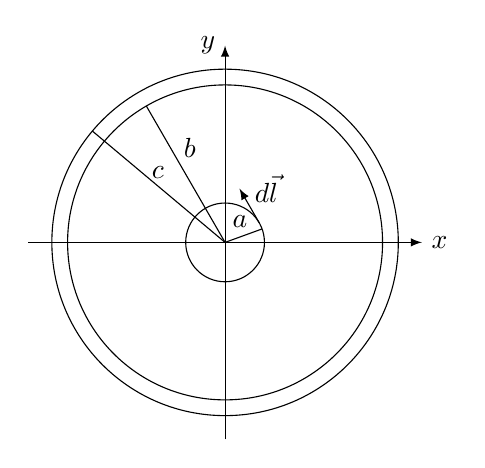
\begin{tikzpicture}
      \draw[-latex] (-2.5,0) -- (2.5,0) node[right]{$x$};
      \draw[-latex] (0,-2.5) -- (0,2.5) node[left]{$y$};

        \draw[] (0,0) -- (20:0.5) node[left=8,above=-3]{$a$};
        \draw[] (0,0) -- (120:2)   node[below=15,right=10]{$b$};
        \draw[] (0,0) -- (140:2.2) node[below=15,right=18]{$c$};
        \draw[-latex] (30:0.5) -- ++(120:0.5)node[right=2]{$d\vec{l}$};

      \draw[] (0, 0) circle (0.5);
      \draw[] (0, 0) circle (2);
      \draw[] (0, 0) circle (2.2);
    \end{tikzpicture}
    \caption{반지름이 $a$인 금속막대와 안쪽 반지름 $b$, 바깥쪽 반지름이 $c$인
    원형 금속관의 단면}
    \label{fig:2}
  \end{figure}

\begin{itemize}
  \item[(가)]
  축으로부터의 거리 $r$이 $a$보다 작은 경우, 반지름이 $r$인 원형 폐곡선을 따라
  생성되는 자기장을 구하자. 페곡선 내부의 면적 $A_{in}$에 흐르는 전류 $I_{in}$은
  반지름이 $a$인 금속막대에 흐르는 전류 $I$와 다음의 관계가 있다.
  \begin{align}
    I_{in} = \frac{A_{in}}{A}I = \frac{\pi r^2}{\pi a^2}I
    = \frac{r^2}{a^2}I.
  \end{align}
  식~\eqref{eq:2-1}에 의하면
  \begin{align}
    \int \vec{B}\cdot d \vec{l}=\mu_0 I_{in}=\mu_0 \frac{r^2}{a^2}I
  \end{align}
  이다. 자기장 $\vec{B}$는 직선 도선이 만드는 자기장이므로 
  $\vec{B}$의 방향은 $d\vec{l}$과 평행하다. 따라서
  \begin{align}
    \int \vec{B}\cdot d \vec{l} = \left|\vec{B} \right|2\pi r
    =\mu_0\frac{r^2}{a^2}I \Longrightarrow
    \left|\vec{B} \right| = \frac{\mu_0 r I}{2\pi a^2}
  \end{align}
  를 얻는다. 자기장의 방향은 $d\vec{l}$와 일치하고 $d\vec{l}$는 각벡터 방향을
  향하므로 자기장 $\vec{B}$는
  \begin{align}
    \vec{B} = \frac{\mu_0 r I}{2\pi a^2}\hat{\bm \phi}
  \end{align}
  이다.
  \item[(나)]
  $a<r<b$인 경우,  폐곡선이 반지름이 $a$인 금속막대의 단면을 모두 포함하므로
  식~\eqref{eq:2-1}을 다음과 같이 쓸 수 있다.
  \begin{align}
    \int \vec{B}\cdot d \vec{l}=\left|\vec{B} \right|2\pi r=\mu_0 I
    \Longrightarrow 
    \left|\vec{B} \right|=\frac{\mu_0 I}{2\pi r}
  \end{align}
  이 경우 역시 자기장의 방향은 $d\vec{l}$와 일치하므로
  \begin{align}\label{eq:2-2}
    \vec{B} = \frac{\mu_0 I}{2\pi r}\hat{\bm \phi}
  \end{align}
  를 얻는다.
  \item[(다)]
  이 경우, 자기장에 중첩의 원리가 적용된다는 사실을 이용하자.
  반지름이 $c$인 단면과 $a$인 단면에 같은 방향으로 전류가 흐르고
  반지름이 $b$인 단면에 반대 방향으로 전류가 흐른다 하여 문제를 풀자.
  먼저, 반지름이 $c$인 단면에 흐르는 총 전류는 원형 금속관일 때 전류가 $I$만큼 
  흐른다는 사실로부터 전류밀도를 구하고 면적을 곱해 구할 것이다.
  반지름이 $c$인 단면에 흐르는 면적 당 전류밀도 $J_c$는
  \begin{align}
    J_c = \frac{I}{\pi(c^2-b^2)}
  \end{align}
  이고 이 단면에 흐르는 총 전류 $I_c$는
  \begin{align}
    I_c = \pi c^2 J_c = \frac{c^2}{c^2-b^2}I
  \end{align}
  임을 알 수 있다. 반지름이 $b$인 단면에 반대 방향으로 흐르는 전류의 전류밀도
  $J_b$는 반지름이 $c$인 단면과 겹치는 부분을 상쇄해야 하므로 반지름이 $c$인
  단면의 전류밀도 $J_c$와 같다.
  \begin{align}
    J_b = J_c.
  \end{align}
  따라서, 반지름이 $b$인 단면에 흐르는 전류 $I_b$는
  \begin{align}
    I_b = \pi b^2 J_b = \frac{b^2}{c^2-b^2}I
  \end{align}
  이다. 우리가 구한 두 전류 $I_b$, $I_c$는 각각 반지름이 $b$, $c$인
  원통형 금속막대에 흐르는 전류이므로 식~\eqref{eq:2-2}을 이용해 
  각 전류에 의해 생성되는 자기장 $\vec{B_b}$, $\vec{B_c}$를 구할 수 있다.
  \begin{align}
    \vec{B_b} &= -\frac{\mu_0 I_b}{2\pi r}\hat{\bm \phi}
    =-\frac{\mu_0 b^2 I}{2\pi r(c^2-b^2)}\hat{\bm \phi}
    , \\
    \vec{B_c} &=  \frac{\mu_0 I_c}{2\pi r}\hat{\bm \phi}
    = \frac{\mu_0 c^2 I}{2\pi r(c^2-b^2)}\hat{\bm \phi}.
  \end{align}
  $\vec{B_b}$는 전류의 방향이 반대이므로 $-$부호가 붙는다. 반지름이 $a$인
  단면에 의해 생성되는 자기장 $\vec{B_a}$는 식~\eqref{eq:2-2}이고
  총 자기장 $\vec{B}$는 이들을 모두 합한 값이다.
  \begin{align}
    \begin{split}
      \vec{B} &= \vec{B_a}+\vec{B_b}+\vec{B_c}
      =\frac{\mu_0 I}{2\pi r}\left[1
      -\frac{b^2 }{c^2-b^2}
      +\frac{c^2 }{c^2-b^2}\right]\hat{\bm \phi}  \\
      &=\frac{\mu_0 I}{\pi r}\hat{\bm \phi}.
    \end{split}
  \end{align}
  $r>c$인 경우에 생성되는 자기장은 각벡터 방향이고 크기는 
  $\frac{\mu_0 I}{\pi r}$이다.

  %이 경우, 원형 금속관의 단면까지 모두 포함하므로 금속막대에 의한 자기장 
  %$\vec{B}_1$와 원형 금속관에 의한 자기장 $\vec{B}_2$를 따로 구하자. 
  %총 생성되는 자기장 $\vec{B}$는 중첩의 원리에 의해 각 자기장을 모두 더한 것과
  %같다.
  %\begin{align}
  %  \vec{B} = \vec{B}_1+\vec{B}_2.
  %\end{align}
  %자기장 $\vec{B}$
\end{itemize}

\vspace{1cm}

\noindent {\bf 문제 3 [30pt].}
그림~\ref{fig:3}처럼 생긴 도선에 전류 $i$가 흐른다. 이 전류는 모양이
똑같이 생긴 두 개의 반원형의 도선으로 나뉜 뒤, 다시 합친다. 이 원형
모양의 도선 중심$C$에서 자기장을 구하여라. 
\begin{figure}[htp]
  \centering
  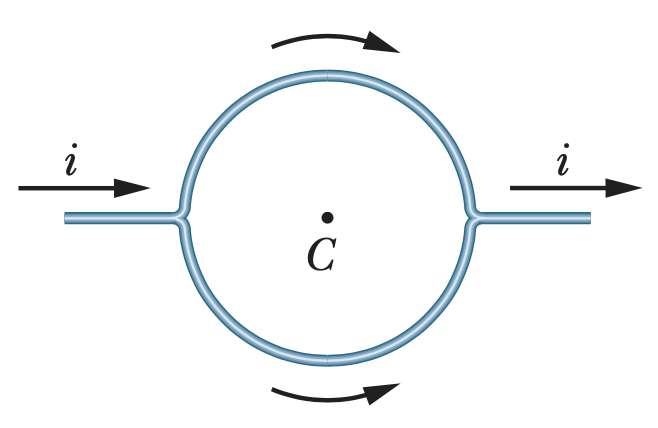
\includegraphics[scale=0.55]{qfig10-1.png}
  \caption{\textbf{문제 3}}
  \label{fig:3}
\end{figure}

\vspace{1cm}
\noindent {\bf 풀이 :} 
도선을 두 부분으로 나누어 각각에 의한 자기장을 생각해보자.
먼저 도선 중심 $C$를 기준으로 왼쪽과 오른쪽에 존재하는 도선에 의한 자기장은
도선의 미소길이 방향 $d\vec{l}$과 미소 도선부터 $C$까지의 단위벡터 $\hat{\bm r}$이
평행하므로
\begin{align}
  d\vec{l}\parallel \hat{\bm r} \Longrightarrow
  d\vec{l}\times \hat{\bm r}=0
\end{align}
이고 비오-사바르 법칙에 의해 자기장도 $0$이다.
이제 원형 도선에 의한 자기장만 따져주면 되는데 윗 도선과 아랫 도선의 전류 방향이
각각 시계 방향, 시계 반대 방향으로 반대이다. 즉, $d\vec{l}$이 반대이다. 윗 도선의
미소길이 방향을 $d\vec{l}_{u}$, 아랫 도선의 미소길이 방향을 $d\vec{l}_{d}$라 
하면
\begin{align}
  \begin{split}
    d\vec{l}_{u} &= -Rd\phi(-\sin\phi\,\hat{\bm i}+\cos\phi\,\hat{\bm j}), \\ 
    d\vec{l}_{d} &= Rd\phi(-\sin\phi\,\hat{\bm i}+\cos\phi\,\hat{\bm j})
  \end{split}
\end{align}
이다. $R$은 두 도선으로 이루어진 원형 도선의 반지름이다. 따라서 두 도선에 의한
자기장은 서로 크기는 같고 방향만 반대가 된다. 중첩의 원리에 의해 총 자기장은
두 자기장을 더한 것이므로 서로 상쇄되고 총 자기장은 $\vec{0}$이다.
\vspace{1cm}

\noindent {\bf 문제 4 [50pt].}
그림~\ref{fig:4}은 반지름이 $a=4.00$ cm인 긴 원통형 도체에 반지름이
$b=1.50$ cm의 긴 원통형 구멍이 도체의 축과 평행되게 나 있는 걸
보여주는 단면이다.  이 구멍의 중심은 원형 도체의 중심에서부터 $d=2.00$
cm 떨어져 있다. 이 원통형 도체에는 전류 $i=5.25$ A가 균일하게 흐르고
있다고 하자. 
\begin{figure}[htp]
  \centering
  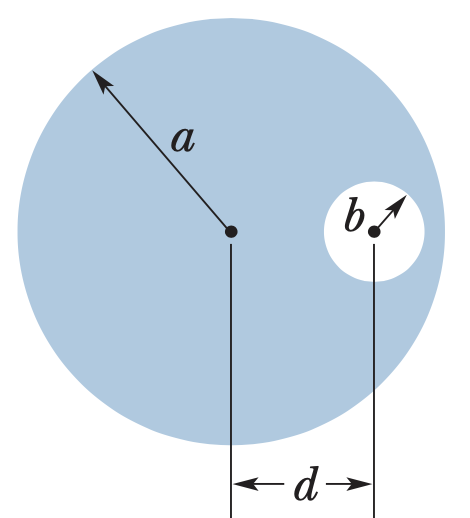
\includegraphics[scale=0.55]{qfig10-3.png}
  \caption{\textbf{문제 4}}
  \label{fig:4}
\end{figure}
\begin{itemize}
\item[(가)] 이 구멍의 중심에서 자기장은 얼마인가?
\item[(나)] $b=0$일 때와 $d=0$일 때의 결과를 구하고 논하여라. 
\end{itemize}

\vspace{1cm}
\noindent {\bf 풀이 :} 
\vspace{1cm}


\end{document}